% Created 2021-04-21 Wed 21:00
% Intended LaTeX compiler: xelatex
\documentclass[12pt]{article}
\usepackage{graphicx}
\usepackage{grffile}
\usepackage{longtable}
\usepackage{wrapfig}
\usepackage{rotating}
\usepackage[normalem]{ulem}
\usepackage{amsmath}
\usepackage{textcomp}
\usepackage{amssymb}
\usepackage{capt-of}
\usepackage{hyperref}
\usepackage{minted}
\usepackage{amsmath}
\usepackage{amssymb}
\usepackage{setspace}
\usepackage{subcaption}
\usepackage{mathtools}
\usepackage{xfrac}
\usepackage[margin=1in]{geometry}
\usepackage{marginnote}
\usepackage[utf8]{inputenc}
\usepackage{color}
\usepackage{epsf}
\usepackage{tikz}
\usepackage{graphicx}
\usepackage{pslatex}
\usepackage{hyperref}

\usepackage{beton}
\usepackage{euler}
\usepackage[OT1]{fontenc}

\usepackage{textgreek}
\renewcommand*{\textgreekfontmap}{%
{phv/*/*}{LGR/neohellenic/*/*}%
{*/b/n}{LGR/artemisia/b/n}%
{*/bx/n}{LGR/artemisia/bx/n}%
{*/*/n}{LGR/artemisia/m/n}%
{*/b/it}{LGR/artemisia/b/it}%
{*/bx/it}{LGR/artemisia/bx/it}%
{*/*/it}{LGR/artemisia/m/it}%
{*/b/sl}{LGR/artemisia/b/sl}%
{*/bx/sl}{LGR/artemisia/bx/sl}%
{*/*/sl}{LGR/artemisia/m/sl}%
{*/*/sc}{LGR/artemisia/m/sc}%
{*/*/sco}{LGR/artemisia/m/sco}%
}
\makeatletter
\newcommand*{\rom}[1]{\expandafter\@slowromancap\romannumeral #1@}
\makeatother
\DeclarePairedDelimiterX{\infdivx}[2]{(}{)}{%
#1\;\delimsize\|\;#2%
}
\newcommand{\infdiv}{D\infdivx}
\DeclarePairedDelimiter{\norm}{\left\lVert}{\right\rVert}
\DeclarePairedDelimiter{\ceil}{\left\lceil}{\right\rceil}
\DeclarePairedDelimiter{\floor}{\left\lfloor}{\right\rfloor}
\def\Z{\mathbb Z}
\def\R{\mathbb R}
\def\C{\mathbb C}
\def\N{\mathbb N}
\def\Q{\mathbb Q}
\def\noi{\noindent}
\onehalfspace
\usemintedstyle{bw}
\author{Sandy Urazayev\thanks{University of Kansas (ctu@ku.edu)}}
\date{52; 12021 H.E.}
\title{Homework 2 Oracle\\\medskip
\large MATH 220 Spring 2021}
\hypersetup{
 pdfauthor={Sandy Urazayev},
 pdftitle={Homework 2 Oracle},
 pdfkeywords={},
 pdfsubject={},
 pdfcreator={Emacs 28.0.50 (Org mode 9.4.5)}, 
 pdflang={English}}
\begin{document}

\maketitle
\href{./index.pdf}{[View the PDF version]​}

\section*{Chapter 2.1}
\label{sec:orgf7e8d8b}
\subsection*{Problem 13}
\label{sec:org9997627}
\begin{center}
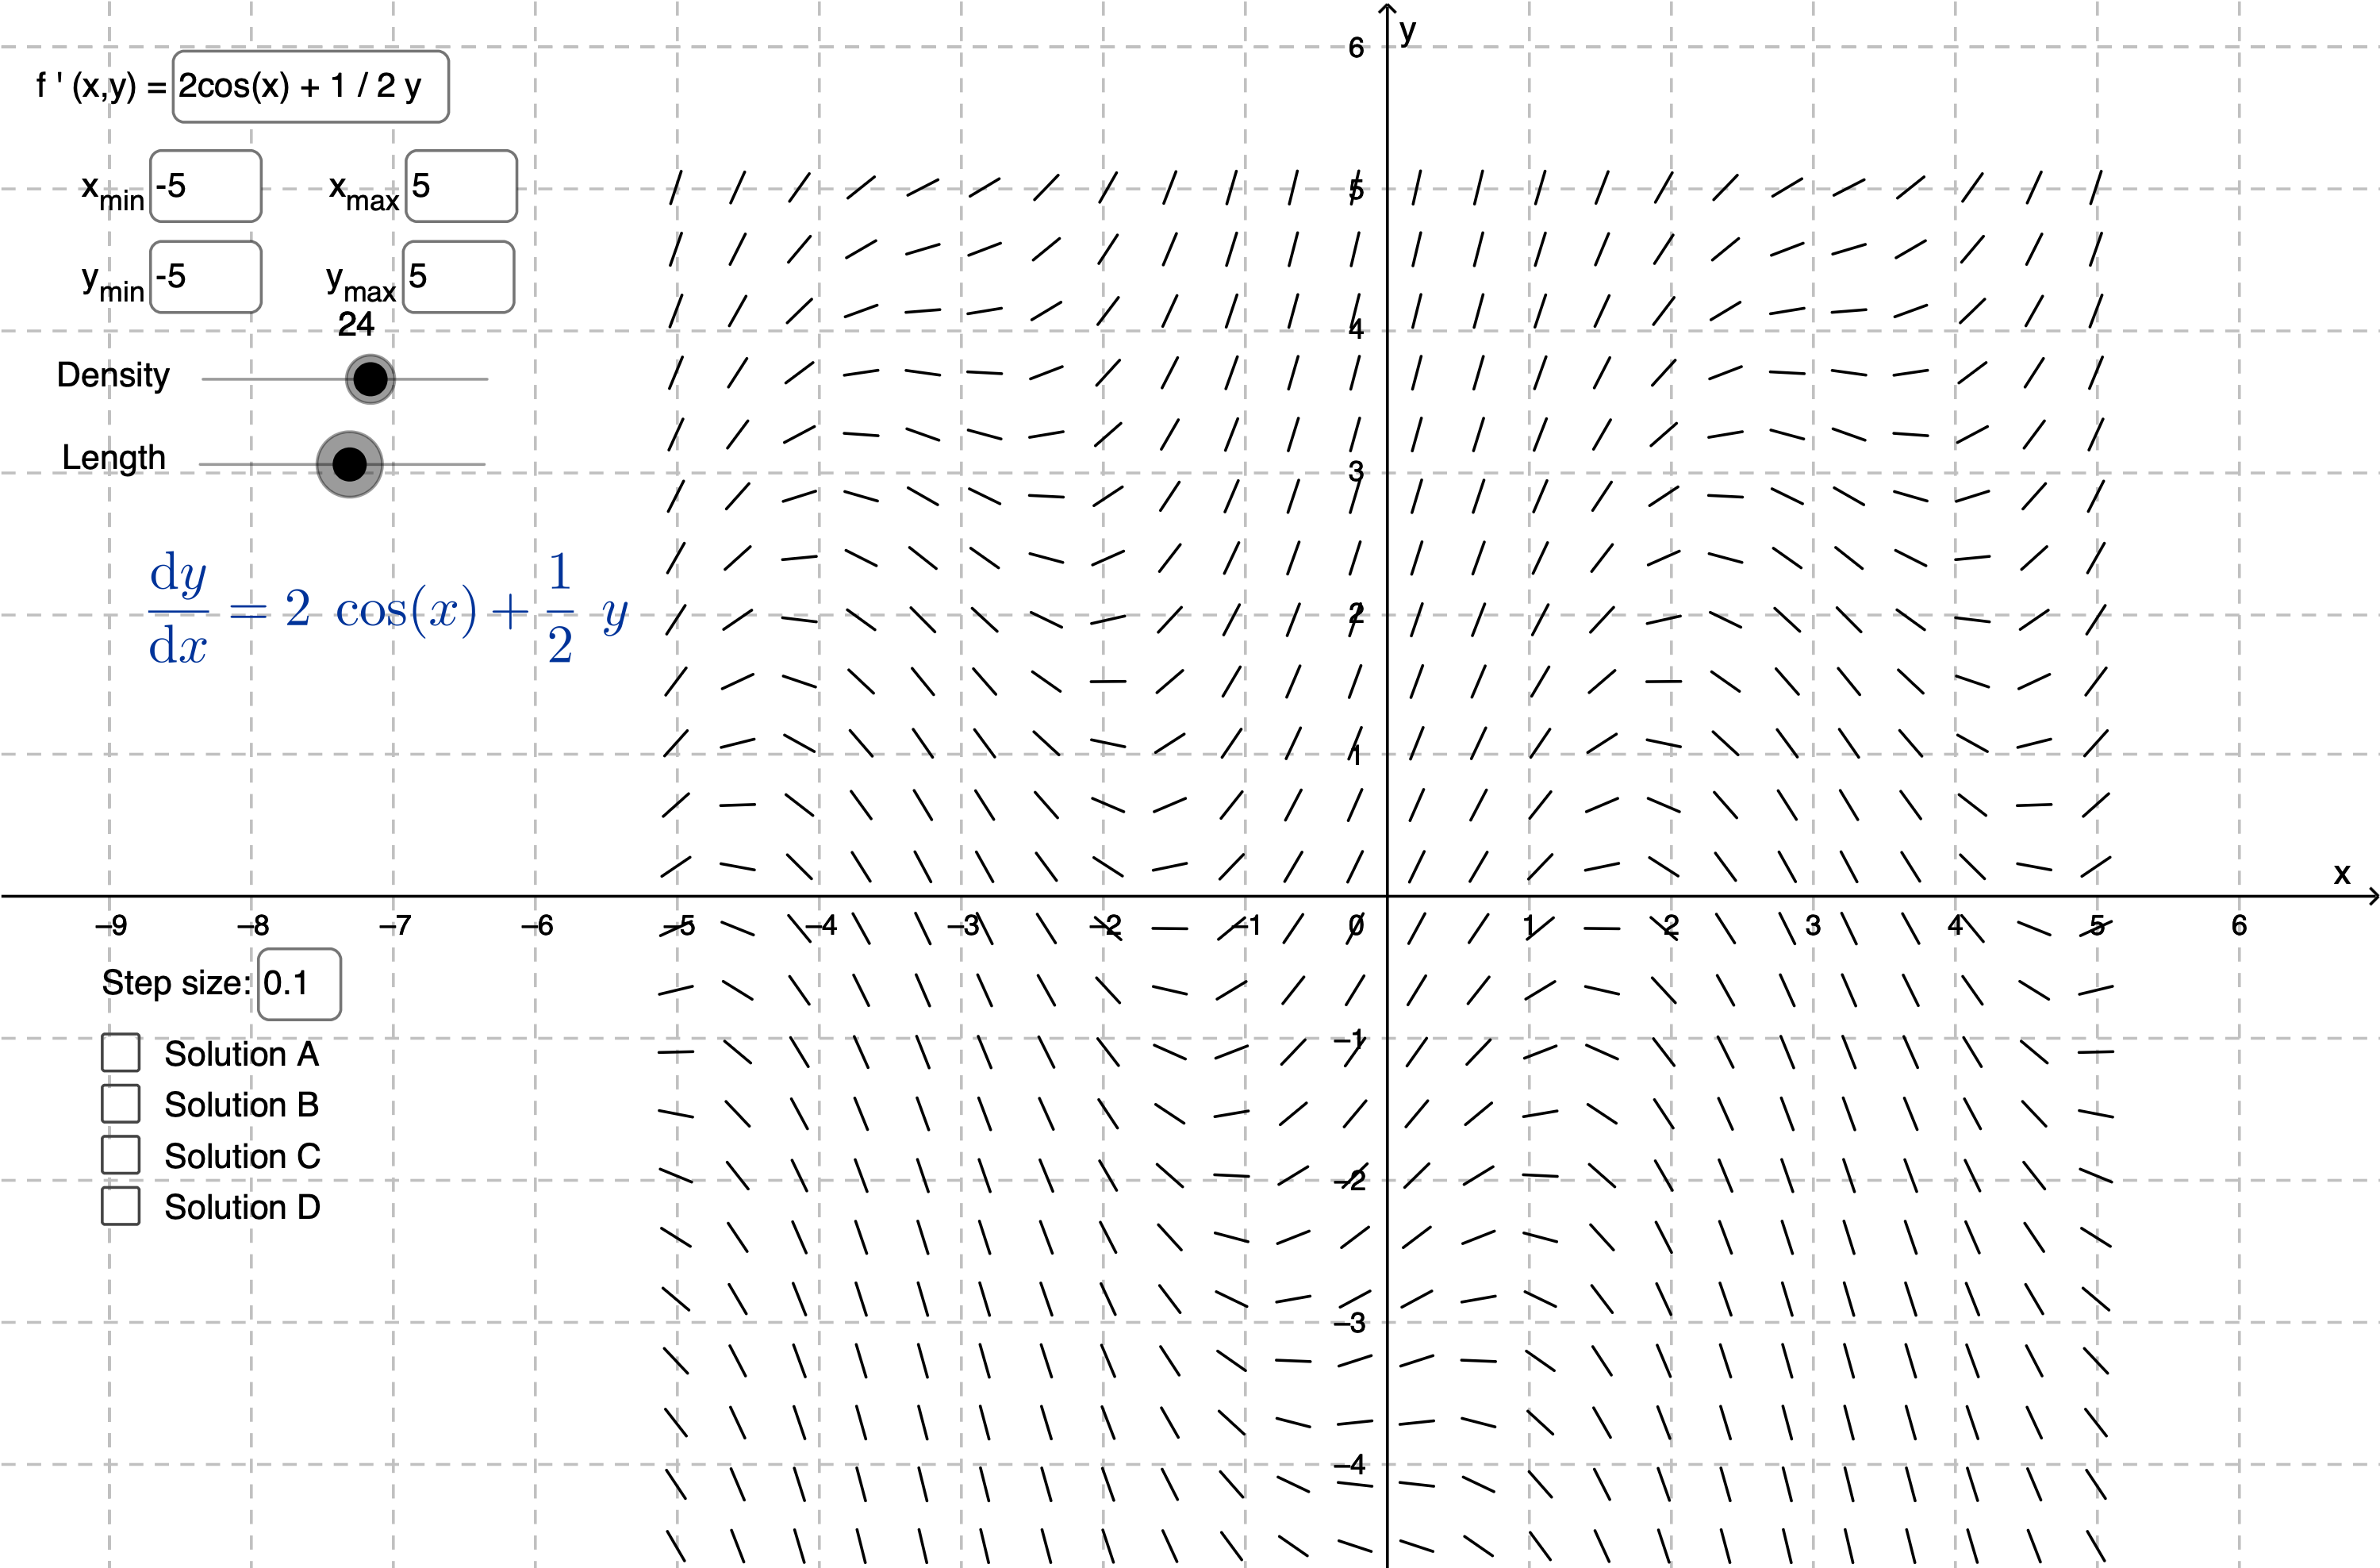
\includegraphics[width=.9\linewidth]{./13.png}
\end{center}
\subsubsection*{Part a}
\label{sec:org69d6c57}
As \(t\) gets infinitely large, it simply oscillates in an inverse cosine
fashion. \(a\) does give the function an initial starting point, to which it
starts oscillating from. That would probably be \(a + \pi\) because
\(2cos(t)\) changes its behaviour every \(\pi\) revolution.
\subsubsection*{Part b}
\label{sec:orgae3c71a}
This is a first-order linear differential equation
of the form \(y' + p(t) y = q(t)\). Find
\(\mu(t) = e^{\int{-\frac{1}{2}}}\) and then solve \(\frac{d}{dt}(\mu(t)y) = q(t) \mu(t)\)
\(\implies y = \frac{\int q(t) \mu(t) dt}{\mu(t)}\). You should get
\begin{equation*}
        y(t) = ce^{t/2}+\frac{8}{5}\sin(t)-\frac{4}{5}\cos(t)
\end{equation*}
Then solving for \(y(0)\) and \(c\), we have the full solution to be
\begin{equation*}
        y(t) = (a+\frac{4}{5}e^{t/2})+\frac{8}{5}\sin(t)-\frac{4}{5}\cos(t)
\end{equation*}
\subsubsection*{Part c}
\label{sec:orgc69bae0}
\(y\) oscillates for \(a=a_0\)
\subsection*{Problem 15 [FOR GRADE]}
\label{sec:orgd44cab6}
\subsubsection*{Part a}
\label{sec:org3f465b1}
This is again, a first-order linear differential equation, so we do our
\(\mu\) and integration from both sides trick. Recognize that we have to
divide everything by \(t\), so that our lead \(y'\) doesn't have a coefficient
and the method for solving this type of equations is applicable.
\begin{equation*}
        ty'+(t+1)y = 2 t e^{-t} \iff y' + (\frac{t+1}{t})y = 2 e^{-t}
\end{equation*}
After cleaning it up, the actual solution process becomes more or less
trivial, \(\mu(t) = e^{\int{\frac{t+1}{t}}} = te^t\). Then we find for \(t>0\)
\begin{equation*}
        y(t) = \frac{ce^{-t}}{t} + e^{-t}t
\end{equation*}
Applying \(y(1) = a\), then we get
\begin{equation*}
        y(t) = te^{-t} + \frac{(ea-1)e^{-t}}{t}
\end{equation*}
We need \(ea-1\) to be equal to zero, then \(a_0 = \frac{1}{e}\)
\subsubsection*{Part c}
\label{sec:orge9f4557}
As \(t \to 0\), then \(y \to 0\). 
\subsection*{Problem 17 [FOR GRADE]}
\label{sec:orgdc7fddf}
Recall the solution to Problem 13. We need to swap the sign on \(p(t)\) and
update the initial value constant solution. We will get
\begin{equation*}
        y(t) = -\frac{9}{5}e^{t/2}+\frac{8}{5}\sin(t)+\frac{4}{5}\cos(t)
\end{equation*}
Set the derivative of \(y\) to \(0\) and solve for \(t\).
\begin{equation*}
  0 = -\frac{9}{5}\times (-\frac{1}{2}) \times e^{t/2}+\frac{8}{5}\cos(t)-\frac{4}{5}\sin(t)
\end{equation*}
You can check the nature of the point by taking \(y''\). Finally, we find that
the local maximum is at \((t, y) = (1.36, 0.82)\). Better approximated values
are accepted.
\subsection*{Problem 20}
\label{sec:orgb0b228a}
The solution process is similar to the problem of 17, you should get a
general solution for \(y\):
\begin{equation*}
        y = -1 - \frac{3}{2}(\sin t + \cos t) + C e^t
\end{equation*}
where \(C\) is a constant. Solving \(y(0) = y_0\) for \(y_0\) yields that
\(C = y_0 + \frac{5}{2}\) so then the solution is \(y_0 = -\frac{5}{2}\).
\subsection*{Problem 28}
\label{sec:orgd983ec4}
\subsubsection*{Part a}
\label{sec:orge45e7f5}
Recall the form \(y' + p(t) y = g(t)\) and solution form of 
\begin{equation*}
        \frac{d}{dt}(\mu(t)y) = g(t) \mu(t)
\end{equation*}
Then if \(g(t)=0\), solution
is \(y = A e^{-\int{p(t)dt}}\)
\subsubsection*{Part b}
\label{sec:org007d8ad}
Simply substitute (50) into (48), perform some trivial Chain Rule and
confirm that
\begin{equation*}
        A'(t) = g(t) \exp\left(\int p(t) dt\right)
\end{equation*}
\subsubsection*{Part c}
\label{sec:orgf326370}
Substitution is mechanical. Prove that variation of parameters works.
\section*{Chapter 2.2}
\label{sec:orgc1623fe}
\subsection*{Problem 1}
\label{sec:orgb6ae5db}
\begin{equation*}
        \frac{dy}{dx} = \frac{x^2}{y}
\end{equation*}
then
\begin{equation*}
        \int y dy = \int x^2 dx
\end{equation*}
So the solution is
\begin{equation*}
        3y^2-2x^3=C
\end{equation*}
It's OK to leave the solution implicitly here, otherwise, the explicit
solution for \(y\) can be very nasty.
\subsection*{Problem 7}
\label{sec:org20d7cfb}
\begin{equation*}
  \frac{dy}{dx} = \frac{y}{x}
\end{equation*}
then
\begin{equation*}
        \int \frac{dy}{y} = \int \frac{dx}{x}
\end{equation*}
Then
\begin{equation*}
        \ln(y) = ln(x) + ln(C) = ln(C\times x)
\end{equation*}
\(C\) is any constant, then \(\ln(C)\) is also a constant.
Finally, \(y = Cx\)
\subsection*{Problem 8 [FOR GRADE]}
\label{sec:org6f61524}
\begin{equation*}
        \frac{dy}{dx} = \frac{-x}{y}
\end{equation*}
then
\begin{equation*}
        \int y dy = - \int x dx
\end{equation*}
Therefore
\begin{equation*}
        y^2 + x^2 = C
\end{equation*}
It's fine if you wrote \(y = \pm \sqrt{C - x^2}\)
\subsection*{Problem 21}
\label{sec:orgbc4d76d}
\begin{equation*}
        y' = \frac{ty(4-y)}{3}, \quad y(0) = y_0
\end{equation*}
\subsubsection*{Part a}
\label{sec:org4c3e447}
As \(t \to \infty\), then \(y \to 4\)
\subsubsection*{Part b}
\label{sec:orge61fe28}
First, you will have to solve the system, which is a first-order separable
ordinary differential equation.  The implicit solution is
\begin{equation*}
        \frac{3}{4} \ln(\frac{4}{4-5}) = \frac{t^2}{2} + C
\end{equation*}
where \(C = \frac{3}{4} \ln(\frac{y_0}{4-y_0})\).

Solve for \(t\), so
\begin{equation*}
  t = \sqrt{\frac{3}{2} \ln\left(\frac{y(4-y_0)}{y_0(4-y)}\right)}
\end{equation*}
Use \(y = 3.98\) and \(y_0 = 0.5\), then \(t \approx 3.29527\).
\subsection*{Problem 25}
\label{sec:orgeb34c07}
\subsubsection*{Part a}
\label{sec:orgfa077cb}
Simple divide both the numerator and the denominator by \(x\).
\subsubsection*{Part b}
\label{sec:org1f71def}
You should get
\begin{equation*}
        \frac{dy}{dx} = v + x \frac{dv}{dx}
\end{equation*}
\subsubsection*{Part c}
\label{sec:org011aaef}
This is simply to show.
\subsubsection*{Part d}
\label{sec:orgec3ba91}
Yet another separable equation, you should get the implicit solution
\begin{equation*}
  x^4 \left| 2 - v \right| \left| v + 2 \right|^3 = C
\end{equation*}
\subsubsection*{Part e}
\label{sec:org0b10f56}
Rearrange to get
\begin{equation*}
        |y+2x|^3 |2x-y| = C
\end{equation*}
\subsubsection*{Part f}
\label{sec:org31a1245}
It's like a 1/x star. 
\end{document}